\documentclass[11pt, a4paper]{article} 

\usepackage[T1]{fontenc}     % We are using pdfLaTeX,
\usepackage[utf8]{inputenc}  % hence this preparation
\usepackage[british]{babel}  
\usepackage[left = 0mm, right = 0mm, top = 0mm, bottom = 0mm]{geometry}
\usepackage[stretch = 25, shrink = 25, tracking=true, letterspace=30]{microtype}  
\usepackage{graphicx}        % To insert pictures
\usepackage{xcolor}          % To add colour to the document
\usepackage{marvosym}        % Provides icons for the contact details

\usepackage{enumitem}        % To redefine spacing in lists
\setlist{parsep = 0pt, topsep = 0pt, partopsep = 1pt, itemsep = 1pt, leftmargin = 6mm}

\usepackage{FiraSans}        % Change this to use any font, but keep it simple
\renewcommand{\familydefault}{\sfdefault}

\definecolor{cvblue}{HTML}{304263}

%%%%%%% USER COMMAND DEFINITIONS %%%%%%%%%%%%%%%%%%%%%%%%%%%
% These are the real workhorses of this template
\newcommand{\dates}[1]{\hfill\mbox{\textbf{#1}}} % Bold stuff that doesn’t got broken into lines
\newcommand{\is}{\par\vskip.5ex plus .4ex} % Item spacing
\newcommand{\smaller}[1]{{\small$\diamond$\ #1}}
\newcommand{\headleft}[1]{\vspace*{3ex}\textsc{\textbf{#1}}\par%
    \vspace*{-1.5ex}\hrulefill\par\vspace*{0.7ex}}
\newcommand{\headright}[1]{\vspace*{2.5ex}\textsc{\Large\color{cvblue}#1}\par%
     \vspace*{-2ex}{\color{cvblue}\hrulefill}\par}
%%%%%%%%%%%%%%%%%%%%%%%%%%%%%%%%%%%%%%%%%%%%%%%%%%%%%%%%%%%%

\usepackage[colorlinks = true, urlcolor = white, linkcolor = white]{hyperref}

\begin{document}

% Style definitions -- killing the unnecessary space and adding the skips explicitly
\setlength{\topskip}{0pt}
\setlength{\parindent}{0pt}
\setlength{\parskip}{0pt}
\setlength{\fboxsep}{0pt}
\pagestyle{empty}
\raggedbottom

\begin{minipage}[t]{0.33\textwidth} %% Left column -- outer definition
%  Left column -- top dark rectangle
\colorbox{cvblue}{\begin{minipage}[t][5mm][t]{\textwidth}\null\hfill\null\end{minipage}}

\vspace{-.2ex} % Eliminates the small gap
\colorbox{cvblue!90}{\color{white}  %% LEFT BOX
\kern0.09\textwidth\relax% Left margin provided explicitly
\begin{minipage}[t][293mm][t]{0.82\textwidth}
\raggedright
\vspace*{2.5ex}

\Large \textbf{Osvaldo Estrada} \normalsize 

% Centering without extra vertical spacing
\null\hfill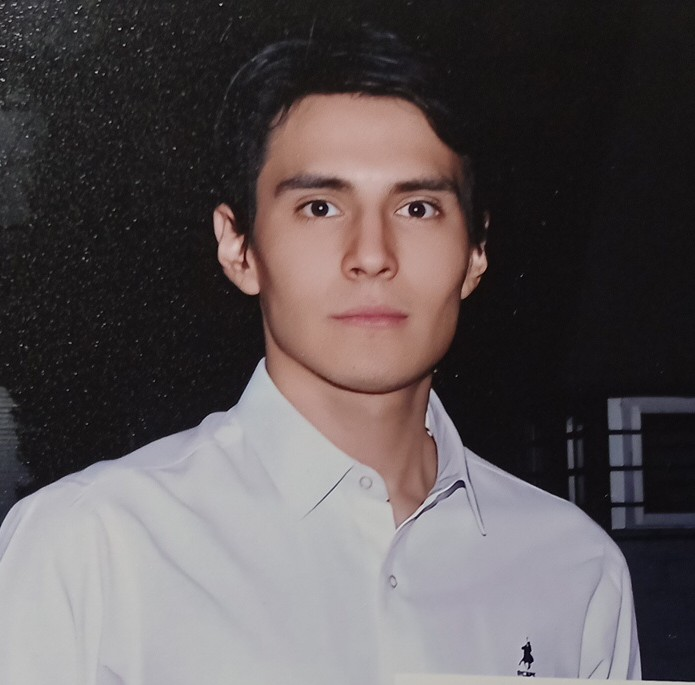
\includegraphics[width=0.65\textwidth]{osvaldo.jpg}\hfill\null

\vspace*{0.5ex} % Extra space after the picture

\headleft{Profile Summary}
A deep love for learning, I am
proactive and organized, consistently
seeking new opportunities to grow.
Result oriented, approaching tasks
with determination and striving for
excellence. Effective communication
is a strength, allowing me to share
ideas clearly and collaborate.


\headleft{Personal information}
Location: \textbf{Mexico, CDMX} \\[0.5ex]
Birth: \textbf{October 20, 2000} \\[0.5ex]
Languages: \textbf{Spanish}, \textbf{English} \\[0.5ex]
Email:\textbf{osvaldoes.unam@gmail.com} \\[0.5ex]
Linkedin: \href{https://www.linkedin.com/in/osvaldo-israel-estrada-sosa-19529919a/}{Click me}

\headleft{Skills}
\begin{itemize}
\item Python, Numpy, Scikit-learn
\item Pyspark, DBT, Azure Databricks
\item Dimensional Modelling, ER Modelling
\item SQLServer, Postgres
\item Flask
\item Git, Github, Bitbucket
\item Linux/UNIX, CLI, Docker
\end{itemize} 

\headleft{Interests}
\begin{itemize}
\item Terraform, Cloud Architecture
\item AWS SDK
\item AWS Certified Data Engineer Associate
\item Snowflake
\item DataOps and CI/CD
\end{itemize}

\end{minipage}%
\kern0.09\textwidth\relax%%Right margin provided explicitly to stretch the colourbox
}
\end{minipage}% Right column
\hskip2.5em% Left margin for the white area
\begin{minipage}[t]{0.56\textwidth}
\setlength{\parskip}{0.8ex}% Adds spaces between paragraphs; use \\ to add new lines without this space. Shrink this amount to fit more data vertically

\vspace{2ex}

\headright{Experience}

\textsc{Data Engineer}\\
\textit{at Exploration \& Discovery Technologies}\\
\dates{November 2023 - }\\
Data Engineer with a proven track record in optimizing data pipelines and improving operational efficiency. Experienced in leveraging technologies such as Python, SQL, Docker, DBT, Databricks, and PySpark. Skilled in data modeling, ETL processes, and CI/CD practices, from development to deployment.

\vspace{0.2cm}
\textsc{Data Scientist}\\
\textit{at Insaite}\\
\dates{July 2022 - February 2023}\\
I have worked on entire data pipelines for churn prediction, medical reports, text classification and decision making dashboards.
Involve in data ingestion, passing through exploratory data analysis, using advanced data engineer manipulations, storing on warehouses and relational databases, finally implementing useful KPIs and machine learning/deep learning models.

\vspace{0.2cm}
\textsc{Data Engineer}\\
\textit{at Instituto de Investigaciones en Matemáticas Aplicadas y Sistemas}\\
\dates{January 2021 - December 2021}\\
Design and implementation of the entire pipeline to extract, clean and analyze Tiktok videos, with help of web scraping techniques. Management, adminstration of linux systems and RDBMS, populate them with object recognition from a convolutional neural network on top of GPUs and finally predict COVID-19 risky scenes according to OMS aimed to diminish infection.

\headright{Education}

\smaller{B.S.E Applied mathematics and computer science}\\
\smaller{Universidad Nacional Autónoma de México}. \dates{2019-2022}

\headright{Certifications}

\smaller{AWS Certified Cloud Practitioner}
\is
\smaller{Databricks Certified Associate Developer for Apache Spark 3.0}
\is
\smaller{Databricks Certified Data Engineer Associate}
\is
\smaller{Scrum Master Certified}

\end{minipage}

\end{document}
